\begin{figure}[t!]
	\centering
\resizebox{0.9\linewidth}{!}{
\renewcommand{\arraystretch}{0.5}
\begin{tabular}{@{}c@{\hskip 0.05cm}c@{\hskip 0.05cm}c@{}}
		{ Input}&
		{w/o $\mathcal{L}_{embed}$}&
		{w/ $\mathcal{L}_{embed}$}&
	
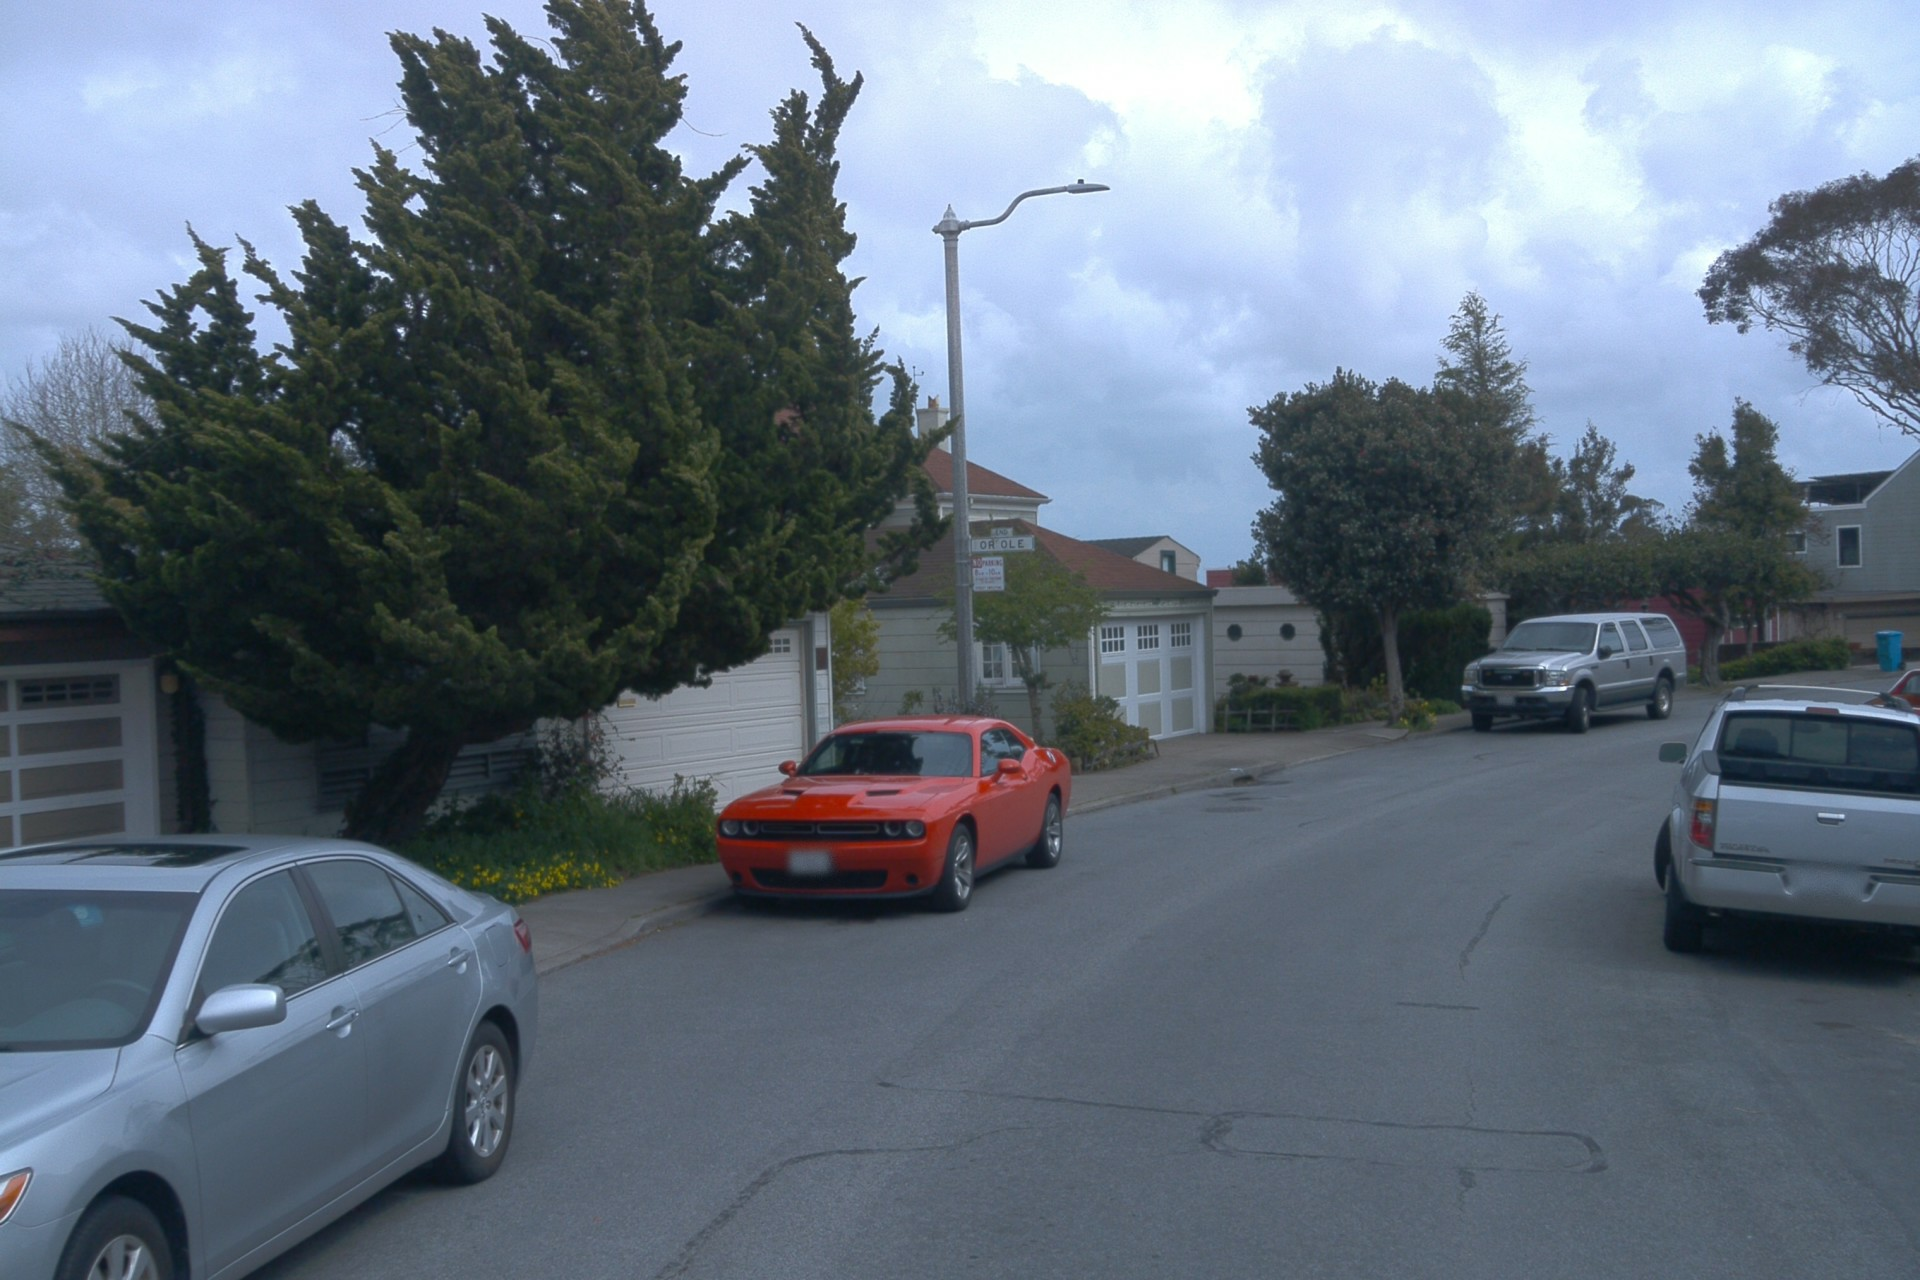
\includegraphics[width=.38\columnwidth, trim={0cm 0cm 0cm 0cm},clip]{fig/optimization_no_trunc_reg/scene2/gt_img.png}&
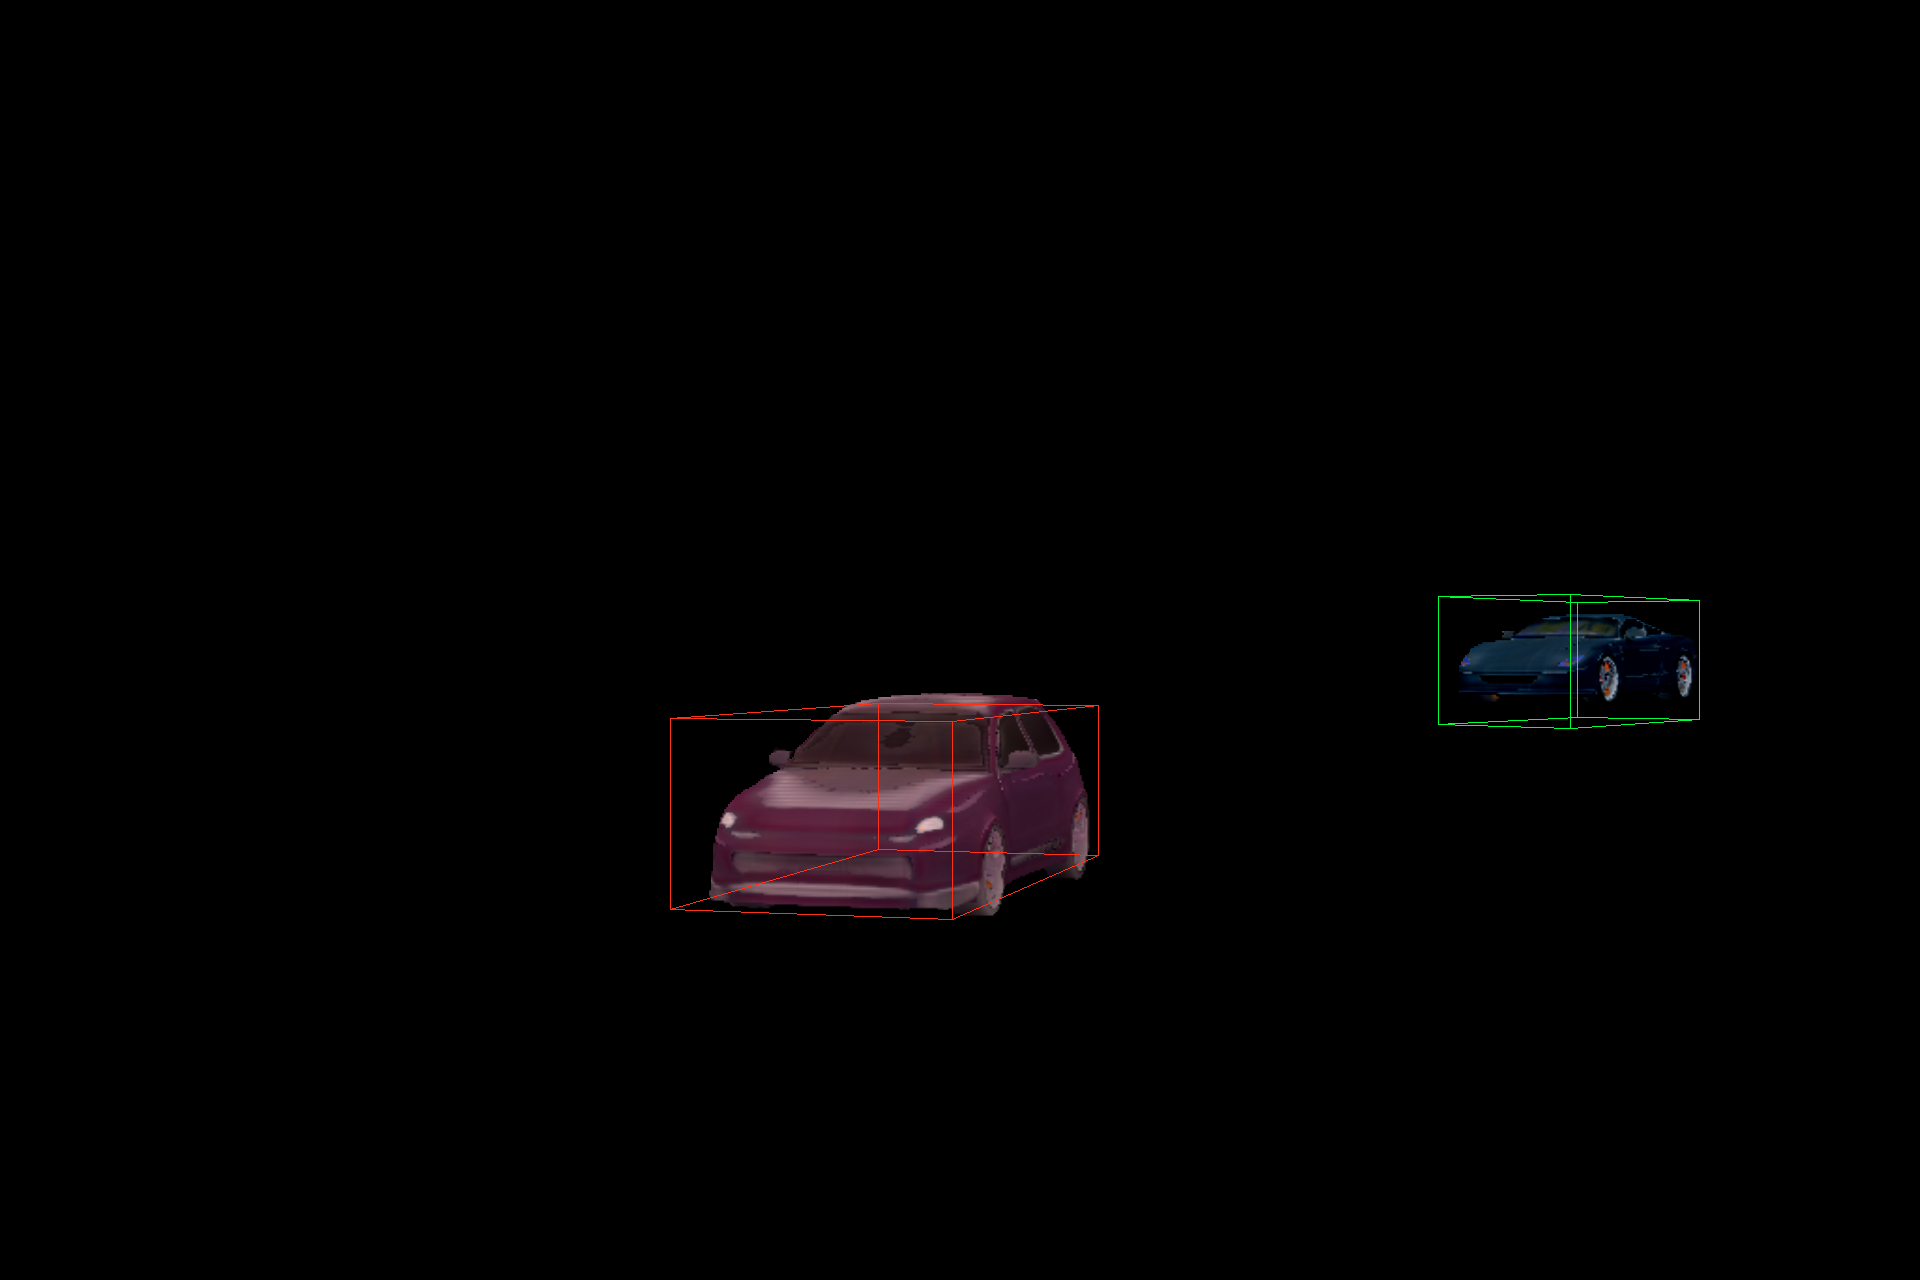
\includegraphics[width=.38\columnwidth, trim={0cm 0cm 0cm 0cm},clip]{fig/optimization_no_trunc_reg/scene2/noembed.png}&
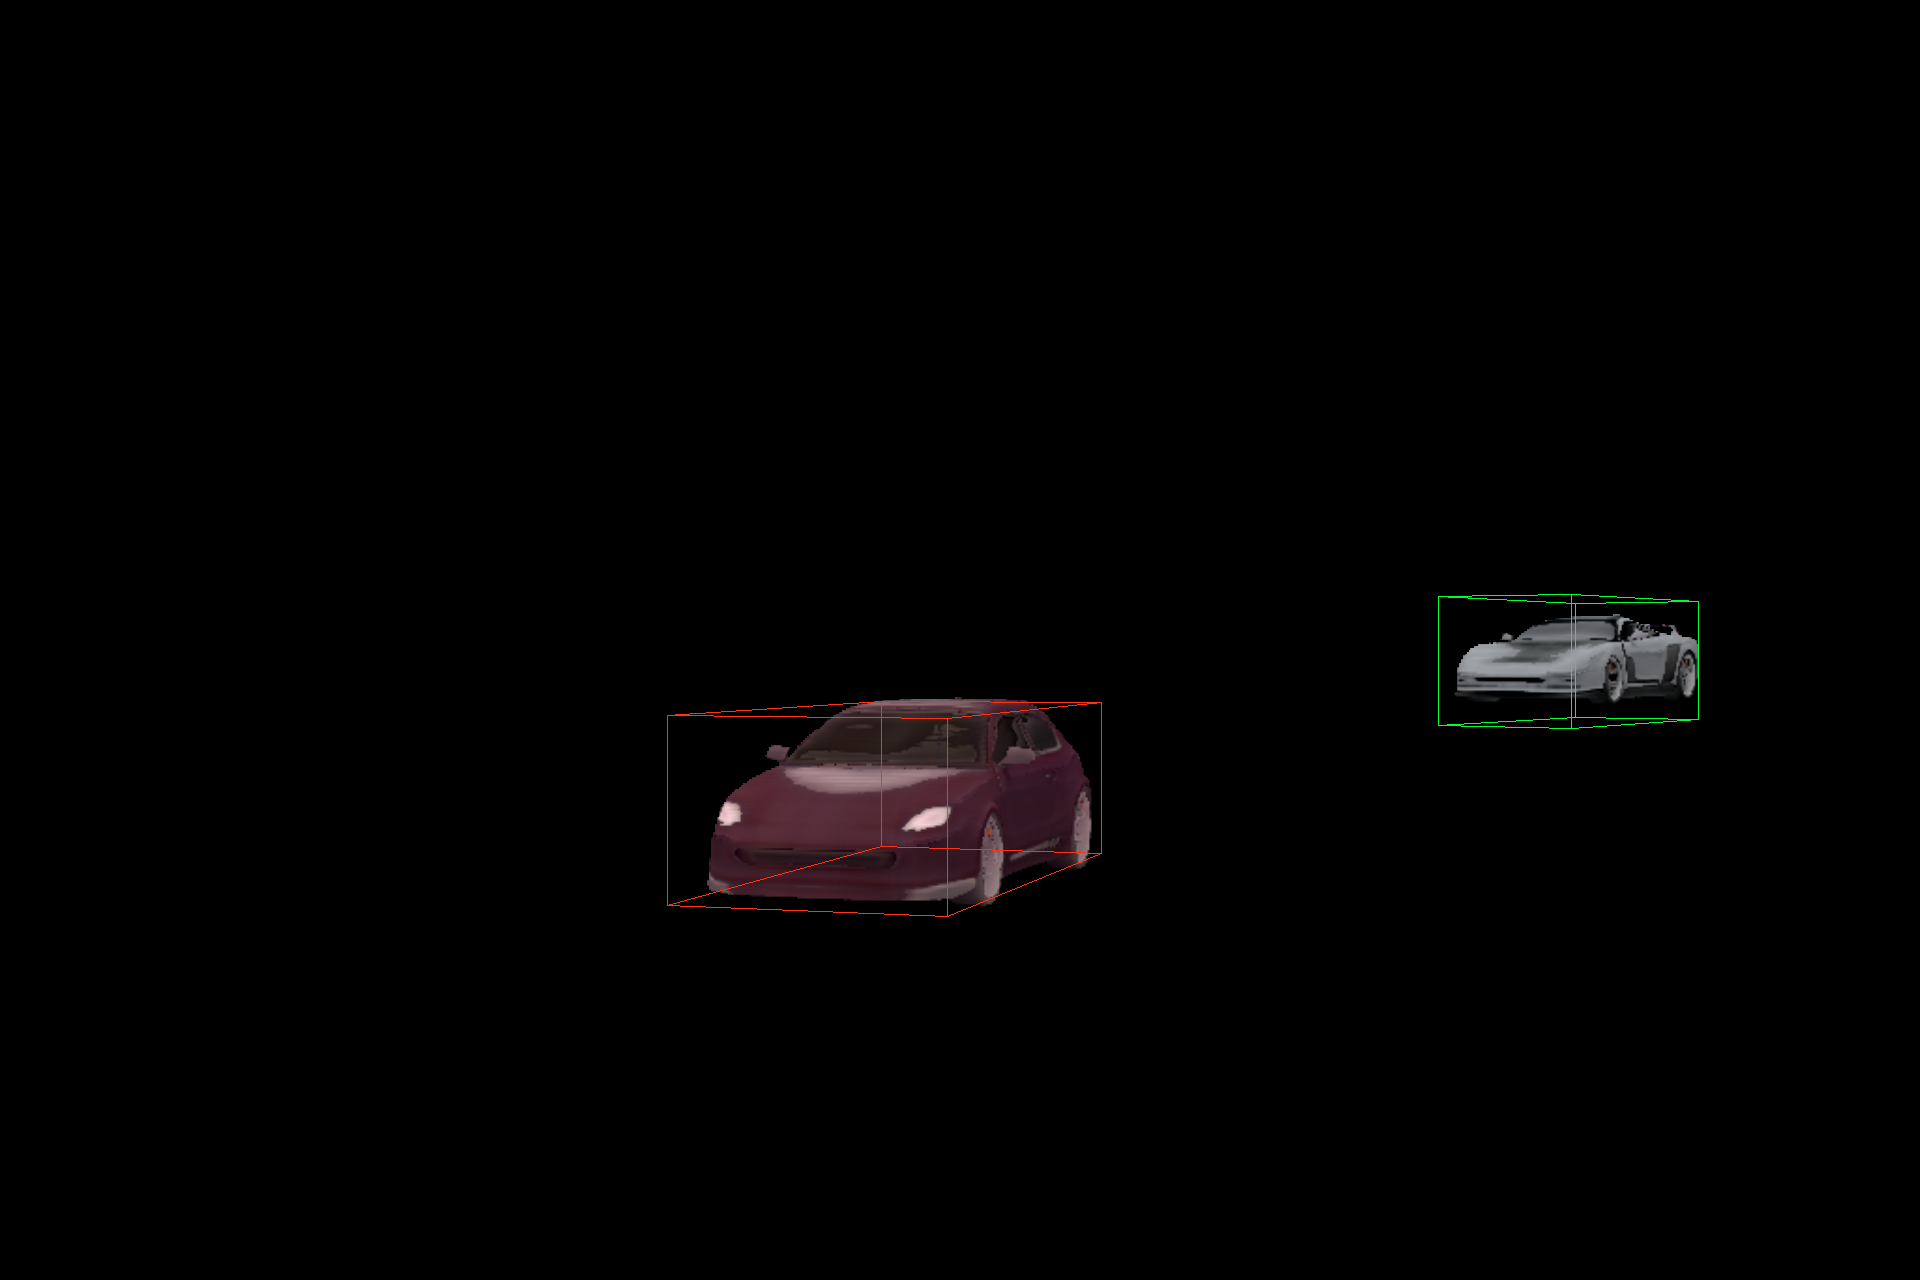
\includegraphics[width=.38\columnwidth, trim={0cm 0cm 0cm 0cm},clip]{fig/optimization_no_trunc_reg/scene2/im_w_bbox_rgb_out.png}
\end{tabular}}
\caption{\textbf{Truncation Trick.} From left to right, (i) The input observed image, (ii) results without truncation regularize applied and (iii) results with a truncation regularize applied. For images (ii) and (iii), we also show bounding boxes for each object color-coded by the respective predicted object IDs. As shown here, applying the truncation regularizer helps us achieve more accurate textures and better shapes and colors for the predicted car surface by forcing the optimized embedding to be ``well behaved'', i.e., close to the distribution of latent embeddings seen during the training by our representation model.}
\label{fig:optimization_truncation}
\end{figure}


